% \section{Conceptos Importantes}



% % \subsection{Sistemas Autónomos} \label{sec:sistemas_autonomos_section}

% % Como se habló previamente en la Sección~\ref{sec:sistemas_autonomos}, los \textbf{Sistemas Autónomos (AS)} son un conjunto de dispositivos que comparten un mismo protocolo de ruteo y están administrados por una misma entidad, cuya interconexión forma \textbf{Internet}.\\

% % Los \textbf{AS} se identifican mediante un número de \textbf{Sistema Autónomo (ASN)} de 16 bits y controlan un conjunto de direcciones \textbf{IP}. 
% % Esta asignación es llevada a cabo por los \textbf{Registros Regionales de Internet} (\textit{Regional Internet Registries}, \textbf{RIRs}), quienes reciben bloques de direcciones IP desde la \textbf{Autoridad Asignadora de Números de Internet} (\textit{Internet Assigned Numbers Authority}, \textbf{IANA}) y los distribuyen a los \textbf{Registros Locales de Internet} (\textit{Local Internet Registries}, \textbf{LIRs}) y a los usuarios finales.\\

% % Los \textbf{Proveedores de Servicios de Internet} (\textit{Internet Service Providers}, \textbf{ISP}), que pueden estar conformados por uno o varios Sistemas Autónomos, se dividen comúnmente en tres niveles de jerarquía:  
% % el \textbf{Tier-1}, donde se encuentran los AS que conforman el \textit{backbone} de Internet y que intercambian paquetes entre sí sin costo asociado;  
% % los \textbf{Tier-2}, generalmente operadores nacionales que compran tránsito a los Tier-1 y venden tránsito a los Tier-3;  
% % y finalmente los \textbf{Tier-3}, operadores locales que pagan por el tránsito para proporcionar acceso a Internet a los usuarios finales~\cite{InterconnectionPeeringSettlements}.  
% % Además, Luckie \textit{et al.}~\cite{ASRank} analizó los AS y propuso una métrica para indicar qué tan global es un AS:  
% % si el \textit{customer cone} es mayor o igual a 200, se considera Tier-1;  
% % si es mayor a 2,000, se considera Tier-2;  
% % y si es menor a 200, se considera Tier-3.\\

% % Una última clasificación que puede hacerse entre AS depende de sus conexiones a otros Sistemas Autónomos, dividiéndolos en \textbf{\textit{single-homed}} y \textbf{\textit{multi-homed}}.  
% % Los AS \textit{single-homed} tienen solo una conexión a otro AS, mientras que los \textit{multi-homed} poseen conexiones a más de un AS.\\









% %--------------------------------------------

% % \subsection{Topología de Internet a nivel de AS} \label{sec:topologia_internt_as_level}


% % Como se ha mencionado a lo largo de esta tesis, el Internet está compuesto por miles de Sistemas Autónomos, los cuales utilizan BGP para intercambiar infomración de ruteo, es decir de alcance entre ello.
% % Así, el Intrnt puede modelarse como un grafo a nivel de AS, donde cada nodo representa un AS, y cada enlace una relacion de conexión dada por BGP (\textit{peering}) entre dos ASes.






% % Zhang et al.~\cite{AS-topology-2004} proponen un método para recolectar la topología de Internet a nivel AS.














% % \subsection{Internet Exchange Points} \label{sec:ixp_section}

% % Los \textit{Internet Exchange Points} (IXPs) son puntos de interconexión donde múltiples ASes pueden establecer relaciones de peering con otros ASes \cite{Computer-Networking}.\\

% % Un IXP consiste generalmente en un switch  o router de alta velocidad y capacidad que conecta routers de diferentes ASes, permitiendo el intercambio directo de tráfico sin necesidad de atravesar redes intermedias. Mejorando así el intercambio de tráfico, haciéndolo más eficiente y de bajo costo.\\

% % % FIXME: arregalr redaccion
% % Las relaciones de tráfico en un IXP se establecen mediante el protocolo BGP, y el IXP solo actua como un intermediario. De esta forma por ejemplo un ISP en vez de estar conectados a multiples ASes  en una coneccion punto a punto, puede conectarse unicamente al IXP y como estos otros ASess tambien estaran conectados al IXP se ahorra recuersos fisicos y de administracion.\\

% % Al igual que los ASes, los IXPs tienen un ASN. Sin embargo, de forma generalizada, este ASN se extrae de los AS PATH en BGP. Algunos IXPs lo mantienen visible como método de debugging \cite{InferringASRelatioships2001}. 

% % \subsection{Mensajes BGP}  \label{sec:anexo_mensajes_bgp}

% % BGP utiliza TCP \cite{RFC793-TCP} como su protocolo de transporte, lo que significa que no necesita preocuparse por la fragmentación de paquetes, la confirmación de recepción (ACK), la retransmisión de datos, entre otros aspectos de confiabilidad.\\

% % Los mensajes BGP solo son procesados una vez que han sido completamente recibidos. Su tamaño mínimo es de 19 octetos, correspondiente al HEADER, mientras que el tamaño máximo es de 4096 octetos. Existen 4 tipos de mensajes en BGP: OPEN, UPDATE, KEEPALIVE y NOTIFICATION.\\


% % \paragraph{Mensaje OPEN}


% % Luego de establecida la conexión TCP entre los pares BGP, el primer mensaje que se envía en un mensaje OPEN ,mediante el cual ambos lados confirman los parámetros de la conexión.
% % En este mensaje se especifica la versión de BGP a utilizar, el número de Sistema Autónomo (AS) del emisor, el Hold Time, el BGP identifier y los parámetros opcionales.
% % El Hold Time define el tiempo máximo que puede pasar sin recibir un mensaje KEEPALIVE o UPDATE en una sesión antes de que la conexión sea cerrada.\\



% % \paragraph{Mensaje UPDATE}

% % Se utiliza para transferir información de enrutamiento entre los pares BGP. A través de este mensaje se anuncian nuevas rutas y se notifican los withdrawals de aquellas que ya no son válidas.
% % Además, estos mensajes incluyen path attributes, los cuales proporcionan información sobre las rutas que se están anunciando para que luego cada AS pueda decidir la mejor ruta a los diferentes destinos. Algunos ejemplos de estos atributos son ORIGIN, AS\_PATH, NEXT\_HOP, MULTI\_EXIT\_DISC, LOCAL\_PREF, ATOMIC\_AGGREGATE y AGGREGATOR.\\



% % \paragraph{Mensaje KEEPALIVE} 

% % El intercambio de mensajes KEEPALIVE dentro del protocolo BGP se utiliza para confirmar que la conexión entre ambos pares sigue activa, evitando que el Hold Time expire.
% % Este mensaje consta únicamente del HEADER de un mensaje BGP, donde se indica que corresponde a un KEEPALIVE por medio del campo \textit{type}, cuyo valor es 2, el cual corresponde al valor 2. Dicho mensaje tiene un tamaño de 19 octetos.\\


% % \paragraph{Mensaje NOTIFICATION}

% % El mensaje \textit{NOTIFICATION} se envía cuando se detecta un error en la comunicación BGP. Una vez enviado, la conexión se cierra.
% % Este mensaje incluye un código de error y un subcódigo de error, los cuales indican en qué tipo de mensaje se produjo el error y la zona específica del problema. Además, contiene un campo de datos que proporciona información adicional sobre el error detectado.\\


% % \subsection{Internet Data collection} \label{sec:anexo_recoleccion_datos_internet}
% % % https:%www.pacnog.org/pacnog17/presentations/MappingTheInternet.pdf

% % La recopilación de datos de Internet es fundamental para comprender su funcionamiento, identificar áreas de mejora y optimizar su infraestructura. La información sobre tráfico, rutas y otros permite detectar anomalías, prevenir amenazas y mejorar el rendimiento global. Además, estos datos son clave para la investigación y el desarrollo de nuevas tecnologías que mejoren la conectividad y la eficiencia de la red.\\

% % A continuación, se presentan algunas fuentes clave que proporcionan datos públicos sobre Internet:\\

% % \subsubsection{CAIDA}

% % El Centro de Análisis de Datos de Internet Aplicados o CAIDA por sus siglas en inglés \cite{CAIDA} es una organización de investigación cuyo principal objetivo es la recopilación y análisis de datos relacionados a la infrestructura, rendimiento y tráfico del Internet. Este funciona como un canal de difusión donde se publican y comparten tanto herramientas como investigaciones relacionado con las redes de Internet.\\

% % En el contexto de nuestro problema de *inferencia de Relaciones entre Sistemas Autonomos*, CAIDA ofrece el dataset *CAIDA AS Relationships* \cite{CAIDAS-relationship}. Este clasifica las relaciones entre Sistemas Autonomos en dos principales tipos: Customer-to-provider (C2P) y Peer-to-peer (P2P). Estas relaciones son inferidas a partir de datos públicos de ruteoBGP ofrecidos por RouteViews \cite{RouteViewsProject} y RIPE RIS \cite{RIPE-RIS}.\\

% % El dataset CAIDA AS Relationships está compuesto por dos subdatasets:
% % \begin{itemize}

% %     \item \textbf{serial-1:} Contiene las relaciones inferidas utilizando un método similar al descrito en el estudio de M. Lukie et al. \cite{ASRank} .Esta disponible desde 1998 hasta la actualidad, con un archivo mensual. Cada archivo incluye un grafo completo derivado de instantáneas de las tablas BGP de RouteViews y RIPE RIS, tomadas cada 2 horas durante un período de 5 días.\\
    
% %     \item \textbf{serial-2:} Basado en el dataset Serial-1, este agrega enlaces inferidos mediante BGP communities, utilizando el método descrito por Vasileios et al. \cite{Inferring-Multilateral-Peering} . Está disponible desde octubre de 2015 hasta el presente, con archivos generados mensualmente.\\
    
% % \end{itemize}

% % Otro proyecto relevante de CAIDA es Archipelago (Ark) Measurement Infrastructure, una plataforma de medición distribuida a nivel global. Esta cuenta con nodos de medición ubicados en diversas zonas geográficas y topológicas para proporcionar una visión integral del estado y funcionamiento de Internet. Entre las mediciones realizadas a través de Ark se encuentran proyectos como The Spoofer Project, Scamper, Internet Topology Discovery, entre otros.\\


% % Además, CAIDA ofrece BGPStream \cite{BGPStream}, una biblioteca de código abierto diseñada para manejar grandes volumenes de datos BGP. Esta herramienta permite acceder tanto a datos BGP en tiempo real como a históricos, obtenidos de los colectores de RouteViews y RIPE NCC. Esto facilita la investigación y el análisis de eventos relacionados con el enrutamiento, como interrupciones, fugas de rutas o ataques BGP, de manera eficiente y rápida.\\


% % \subsubsection{RouteViews Project}

% % El proyecto RouteViews \cite{RouteViewsProject} de la Universidad de Oregon nació en un principio como una herramienta los operadores de Internet, con el fin de que estos pudiesen obtener información BGP en tiempo real sobre el sistema de enrutamiento global desde las perspectivas de varios backbones y ubicaciones en Internet. \\

% % Sin embargo hoy en dia, su uso se ha extendido a multiples tareas, tales como la visualización de rutas AS, el estudio de la utilización del espacio de direcciones IPv4 y  otros aspectos relacionados a la infraestructura y enrutamiento de Internet. \\

% % % Hoy en día, RouteViews es ampliamente utilizado en investigaciones sobre la infraestructura y el comportamiento del enrutamiento global.

% % % TODO: Arreglar ANexo
% % El proyecto cuenta con alrededor de 41  recolectores de enrutamiento  (ver en ANEXO)  ubicados en puntos clave alrededor del mundo, como Ámsterdam, Londres, Sídney, Singapur, São Paulo, Santiago, Nairobi, Sudáfrica, Chicago, California y otras ubicaciones, especialmente en Internet Exchange Points (IXP). Estos recolectores obtienen información de enrutamiento de más de 260 organizaciones diferentes que comparten sus datos  con RouteViews, incluyendo muchos de los ISP más grandes del mundo.\\

% % Los recolectores establecen sesiones de peering BGP con diferentes sistemas autónomos, a través de estas conexiones, los recolectores reciben actualizaciones de las tablas BGP (RIS) y UPDATES del protocolo BGP, obteniendo así información sobre las rutas globales y las conexiones entre AS.
% % En estas actualizaciones incluyen información como:
% % \begin{itemize}
% %     \item \textbf{AS Path:} Camino de Sistemas Autonomos que un paquete debe seguir para llegar a una red destino.
% %     \item \textbf{Prefijos IP:} Rangos de direcciones IP que están siendo anunciados por los AS.
% %     \item \textbf{Next Hop:} Siguiente salto (router o red) que los paquetes deben tomar para continuar hacia su destino.
% % \end{itemize}


% % El proyecto también cuenta con una compilación de archivos en dos formatos, los obtenidos por Cisco y por el software de enrutamiento FRR. El primero recopila información en intervalos de 2 horas, comenzando a las 00:00 UTC. El segundo obtiene RIBs y actualizaciones, los RIBs corresponden a snapshots recogidas cada 2 horas, mientras que los Updates son archivos continuos que se actualizan cada 15 minutos. Estos archivos históricos están en formato MRT y están disponibles para cada recolector.\\


% % % + http:%www.routeviews.org/
% % % + PAPERS: https:%www.routeviews.org/routeviews/index.php/papers/

% % \subsubsection{RIPE NCC RIS}

% % RIPE (Reseaux IP Européens) Network Coordination Centre es uno de los cinco Registros Regionales de Internet (RIRs) que proporciona servicios de registro de Internet y coordinación de recursos de Internet para Europa, Oriente Medio y partes de Asia Central.
% % RIPE NCC opera el Routing Information Service (RIS) \cite{RIPE-RIS}, una plataforma de recopilación de datos de enrutamiento, que tiene como objetivo mejorar la comprensión y visibilidad del sistema global de enrutamiento de Internet.\\

% % Al igual que RouteViews, RIS recopila datos a través de un conjunto de más de 26 colectores (ANEXO) remotos de rutas (RRCs) distribuidos globalmente, generalmente ubicados en Puntos de Intercambio de Internet (IXPs).  Voluntarios se conectan con los RRCs mediante BGP, y RIS almacena los mensajes que recibe de estos peering.\\

% % Para acceder a los datos, existen dos formas: directamente a través de archivos en formato MRT, RIS Live y RISwhois, o mediante herramientas que utilizan los datos de RIS, como RIPEstat, donde se puede encontrar información ya organizada, como la exploración del enrutamiento por país y la localización de información de contacto sobre abusos.\\


% % \subsubsection{PeeringDB}

% % PeeringDB (\cite{PeeringDB}) es una base de datos pública y de acceso libre, gestionada y promovida por voluntarios. Su objetivo principal es facilitar la interconexión entre redes, proporcionando información detallada sobre operadores de red, proveedores de tránsito, centros de datos y Puntos de Intercambio de Internet (IXPs). Gracias a su contenido, es una fuente valiosa para la comunidad de Internet y para investigaciones relacionadas con el enrutamiento y la interconexión de redes. \\

% % PeeringDB contiene una amplia variedad de información, incluyendo los números de Sistema Autónomo (ASN), las políticas de peering, las ubicaciones de redes y los detalles de los IXPs, como la cantidad de participantes y las entidades que los operan. \\























% % Así, la esencia detrás del uso de GNNs radica en su capacidad de entrenar un modelo que pueda procesar un grafo, sus nodos y relaciones, logrando identificar patrones relevantes en la topología para lograr de forma efectiva la tarea asignada.


% % El diseño de una GNN se hace por medio de la combinación de diferentes módulos: 

% % - Módulo de propagación: Este módulo se utiliza para propagar información entre los nodos capturando tanto la topología como los atributos de los nodos. Esto se logra combinando los datos de cada nodo con los de sus vecinos.

% % - Módulo de muestreo: Cuando los grafos son muy grandes, se utiliza generalmente un módulo de muestreo con el fin de seleccionar un subconjunto del grafo, aportando de este modo  en la capacidad de generalización de un modelo y reducción de complejidad. Se combina generalmente con un módulo de propagación.

% % - Módulo de pooling: Cuando se necesita representaciones de subgrafos su utiliza este módulo para extraer información de los nodos. Se utiliza para reducir la dimensionalidad de las representaciones de nodos. 

% % Un modelo GNN se construye generalmente combinando estos módulos. A continuación ( \cite{pipelineGNN}), se ilustra el pipeline de una arquitectura GNN. 
% % El modelo recibe como entrada un grafo, y en la capa GNN, se emplea un operador convolucional, un módulo de muestras y una operación skip-connection que se fusionan para propagar la información y extraer detalles de alto nivel mediante el módulo de pooling. Después de pasar por todas las capas intermedias, se obtiene una salida en forma de embeddings, a los cuales se les aplica una función de pérdida para obtener los resultados del ajuste del modelo en base a la tarea asignada.


% % #figure(
% %   image("../imagenes/basepipelineGNN.png", width: 60%),
% %   caption: [Pipeline básico de una arquitectura GNN.],
% % ) <pipelineGNN>





% \section{Metodos de Inferencia} \label{sec:anexo_inferencia_relaciones_as}

% A continuación se presentan algunos de los métodos desarrollados para la tarea de inferencia de relaciones económicas que comparten los Sistemas Autónomos



% \subsection{Gao}

% El algoritmo presentado por Gao fue el primero en abordar el problema de inferencia de los tipos de relaciones entre Sistemas Autónomos a partir de tablas de enrutamiento BGP y la heurística de los grados de cada AS.

% Para validar sus resultados, Gao utilizó información interna de AT\&T y datos del servicio WHOIS para verificar relaciones de tipo siblings. En este análisis, el 99.1% de los resultados de inferencia fueron confirmados por AT&T.



% Su algoritmo consistió en :
% \begin{enumerate}
%     \item \textbf{Parsear las Routing Tables:} Se parsean las tablas de enrutamiento BGP y se calcula el grado de cada AS.
%     \item \textbf{Identificar el top provider:} Se identifica el top provider de cada AS path.
%     \item \textbf{Clasificar las relaciones:} Se clasifican las relaciones entre los ASes en base a la jerarquía de los ASes y el top provider.
% \end{enumerate}

% La clasificación de relaciones estaba dado por la lógica de que una vez encontrado el top provider de un as path, los pares AS que se encontraran antes del top provider tendrían una relación de P2C, mientras que los pares que se encontraran después del top provider tendrían una relación de P2P y relación S2S si ambos pares proveian de transito para el otro, es decir, podia encontrarse ese par tanto antes como después del top provider.\\

% % FIXME: DEfinir quee es un speaking router
% Pero como no se puede asumir que todos los routers de enrutamiento que pertenecen a un AS estén bien configurados, Gao propuso una mejora para evitar inferencias incorrectas, la cual consistía en contar el número de tablas de enrutamiento que concluyeran que una relación era de un tipo y otra. Es decir, si no más de L tablas de enrutamiento inferían que un AS $u$ proveía de tránsito a AS v y más de L tablas de enrutamiento inferían que $v$ proveía de tránsito a $u$, entonces se ignoraba que u proveía de tránsito a $v$, siendo $L$ una constante pequeña.\\

% En el caso de las relaciones de P2P, Gao primero identificó aquellos ASes con los que no podría establecer relaciones de peering, basándose en la idea de que en una relación de peering los ASes no difieren más de R veces.\\

% \subsection{Lu Rank}

% Uno de los algoritmos más recientes es el propuesto por Ruan y Susan en 2014 \cite{computing-observed-autonomous-system-relationships-in-the-internet}. Hasta ese momento, la mayoría de los métodos para inferir los tipos de relaciones entre sistemas autónomos se basaban en la suposición de que todos los ASes siguen una política uniforme de exportación de rutas. Según esta política, las rutas provenientes de proveedores y peers no son exportadas a AS vecinos que también son proveedores o peers. Bajo este idea, todos los AS Paths serían \textit{valley-free}. \\

% Los algoritmos previos asumían que todos los AS paths eran \textit{valley-free} o buscaban maximizar el número de caminos que cumplían esa propiedad. Sin embargo, se sabe que un gran número de AS paths en los updates  o tablas de enrutamiento BGP no son \textit{valley-free}. Esto hace que al depender de dicha propiedad las relaciones inferidas sean imprecisas.\\

% Ruan y Susan en lugar de basarse en la propiedad de \textit{valley-free}, propusieron un método para clasificar las relaciones observadas entre AS, sustentándose en las relaciones de tránsito entre ellas, a tarves de los datos de BGP. A diferencia del algoritmo de Gao \cite{InferringASRelatioships2001}, que se basa principalmente en el grado de los AS, este método utiliza el concepto de grado de tránsito de los AS lo cual en conjunto con la identificación de los top providers de los AS Path, permiten identificar las relaciones entre AS.\\

% El algoritmo propuesto consta de tres fases principales:
% \begin{enumerate}
%     \item \textbf{Preprocesamiento de los datos:} La entrada consiste en un conjunto de BGP routing table dumps obtenidos de RouteViews \cite{RouteViewsProject}. Estos datos se sanitizan eliminando loops, descartando ASN inválidos, eliminando ASN duplicados y excluyendo conjuntos de ASN terminales, en caso de que estén presentes en las secuencias.
    
%     \item \textbf{Procesamiento de AS paths que contienen AS Tier-1:} 
%     En esta fase se definen dos contadores cnt(X, Y) y cnt(Y, X), los cuales indican el número de veces que X actúa como proveedor de tránsito para Y, y el número de veces que Y actúa como proveedor de tránsito para X respectivamente. Si X e Y aparecen en un AS path antes del top provider, se interpreta que Y proporciona tránsito a X; de lo contrario, X proporciona tránsito a Y. A partir de esta información y la identificación de ASN Tier-1, las relaciones se clasifican en base a las siguientes reglas:


%     \begin{itemize}
%         \item Si $cnt(X, Y) > 0$ y $cnt(Y, X) = 0$, se establece una relación P2C entre X y Y.
%         \item Si $cnt(X, Y) > 0$ y $cnt(Y, X) > 0$, y al menos uno entre X o Y es un AS Tier-1, la relación entre ellos es P2P.
%         \item Si $cnt(X, Y) > 0$ y $cnt(Y, X) > 0$, y ninguno de los dos es un AS Tier-1, la relación es S2S.
%     \end{itemize}


%     \item \textbf{Clasificación de AS paths indeterminados:} En esta fase final, primero se determina el top provider de los AS paths donde no se encontraron AS Tier-1. Para ello, se construye un grafo dirigido en el que cada nodo tiene un atributo denominado \textit{distance}, que indica el camino  más corto en hops a un AS Tier-1. Luego, con esta información al igual que en la fase anterior se puede determianr las relaciones de los AS paths bajo las siguientes reglas:

%     \begin{itemize}
%         \item Si $cnt(X, Y) > 0$ y $cnt(Y, X) = 0$, entonces X y Y tienen una relación provider-to-customer (P2C).
%         \item Si $cnt(X, Y) > 0$ y $cnt(Y, X) > 0$, entonces X y Y tienen una relación peer-to-peer (P2P).
%     \end{itemize}
%   Esta última regla puede corresponder también a una relación S2S, en caso de que en el paso anterior se hayan clasificado como S2S. Si un AS path contiene una relación P2P que no es adyacente a un top provider, entonces se reclasifica como S2S, dado que el enlace es visible a través de un upstream provider. En caso contrario, se mantiene como P2P.


% \end{enumerate}


% \subsection{BGP2Vec}  \label{sec:anexo_bgp2vec}

% En 2020, Tal Shapira y Yuval Shavitt presentaron un nuevo enfoque \cite{UnveilingtheTypeRelationshipBetweenAutonomousSystemsUsingDeepLearning}, para la inferencia de Sistemas Autónomos utilizando por primera vez técnicas de Deep Learning. Este método se basa en la creación de embeddings de estos Sistemas Autónomos utilizando únicamente anunanuncios BGP provenientes de datasets públicos.
% El modelo alcanzó una precisión del 95.8 \% en la clasificación de relaciones entre ASes.\\

% El pipeline que siguieron para esta tecnica consistió en dos etapas: La 
% primera, donde se entrena un modelo de Deep Learning para generar embeddings de los ASes, y la segunda, donde se entrena un modelo de Deep Learning para clasificar las relaciones entre los ASes.\\


% El entrenamiento de BGP2Vec para la generación de embeddings de Sistemas Autónomos consiste en utilizar como entrada un vector one-hot representante del ASN (Número de Sistema Autónomo) y como salida otro vector one-hot que representa los ASNs del contexto. Luego mediante el descenso de gradiente, se ajustan los pesos de la red para maximizar la probabilidad logarítmica de cualquier ASN de contexto dado el ASN de entrada.\\


% \begin{figure}[h]
%     \centering
%     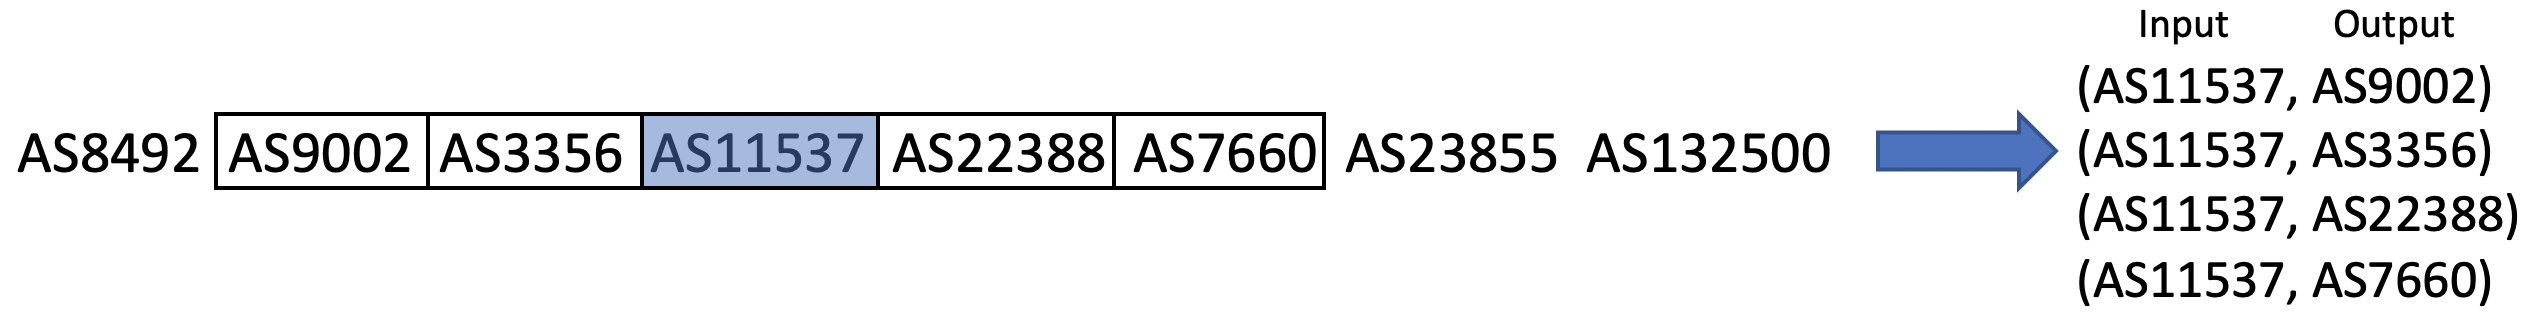
\includegraphics[width=10cm]{img/metodosASRel/BGP2Vec1.png}
%     \caption{Proceso de generación de \textit{embeddings} en BGP2Vec a partir de las RIBs utilizando el modelo Skip-gram.}
%     \label{fig:BGP2Vec-AS-Path}
% \end{figure}

% Una vez entrenado los embeddings para cada ASN, se continúa con la tarea de clasificación de las relaciones entre los Sistemas Autónomos. Para esto se ocupa una Red Neuronal Artificial de dos capas.


% \begin{figure}[h]
%     \centering
%     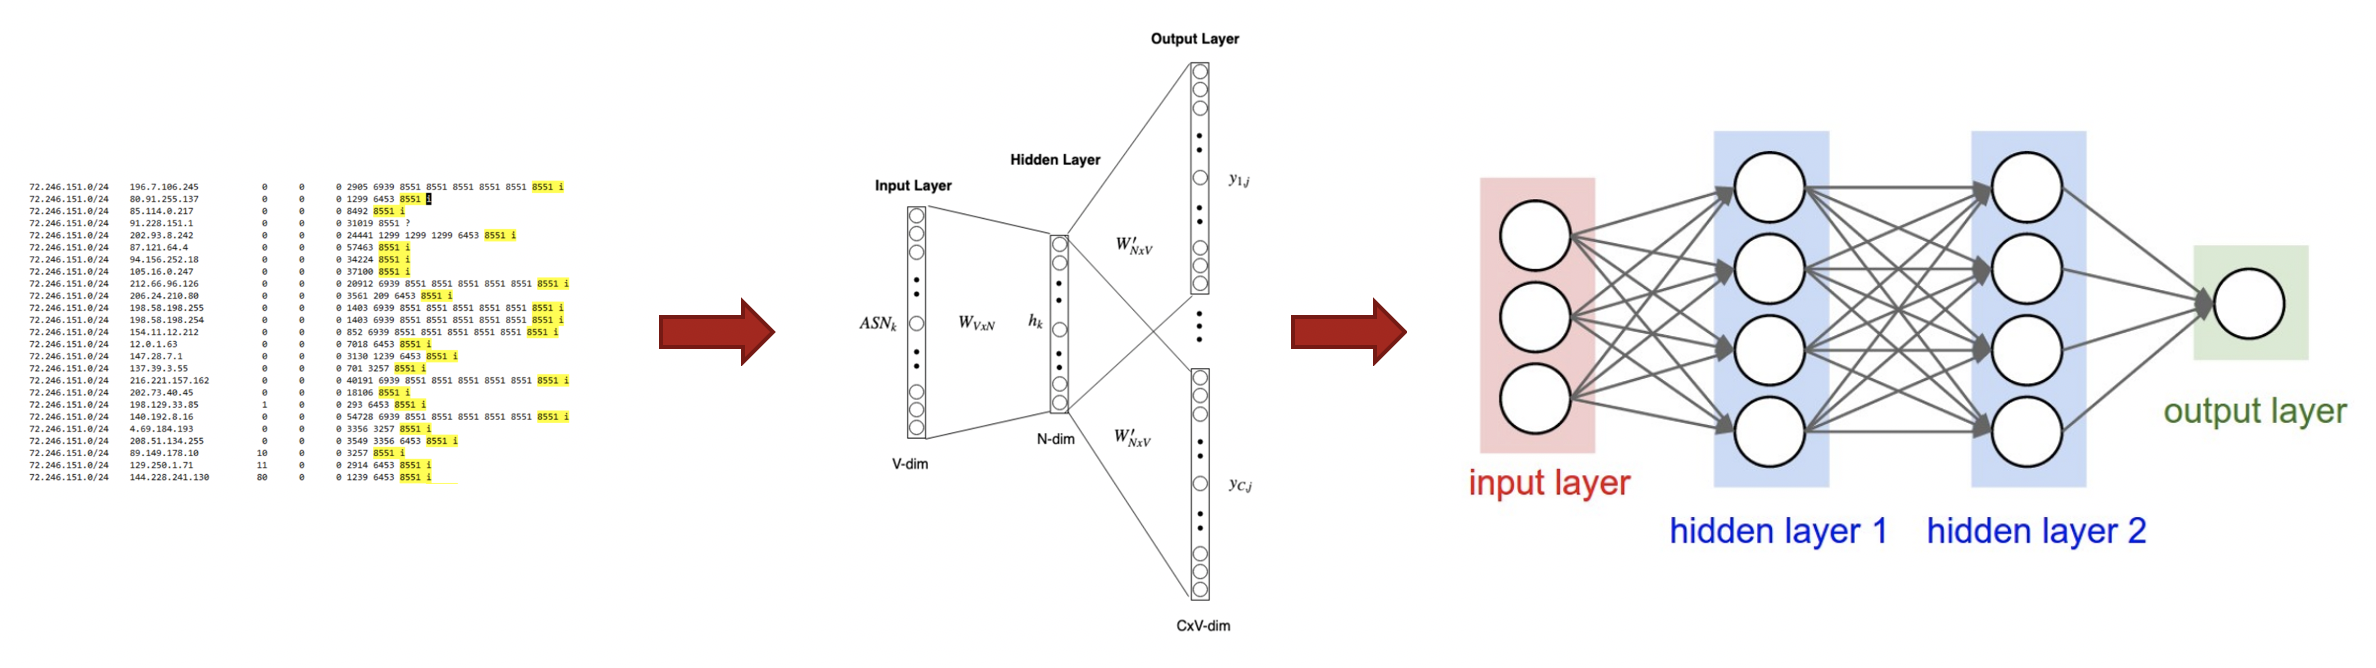
\includegraphics[width=10cm]{img/metodosASRel/BGP2Vec2.png}
%     \caption{Pipeline empleada por estudio BGP2Vec para clasificar las relaciones entre Sistemas Autónomos. Primero a partir de RIBs se crean sus \textit{embeddings} y luego una ANN actúa como clasificador.}

%     \label{fig:BGP2Vec-Pipeline}
% \end{figure}


% Para la etapa inicial de entrenamiento de BGP2Vec, se utilizaron anuncios extraídos de RouteViews \cite{RouteViewsProject}, que contenían anuncios de rutas de AS (AS PATH) recolectadas por 19 colectores. Este dataset recopiló 3,600,000 rutas de AS con 62,525 vértices de AS y 113,400 enlaces no dirigidos.

% Para el entrenamiento de la Red Neuronal encargada de la clasificación de las relaciones entre ASes, se utilizó el conjunto de datos de relaciones entre AS de CAIDA \cite{CAIDAS-relationship}, que contiene relaciones P2P y P2C/C2P. Además, para algunos experimentos, se empleó el dataset ToR de BGProtect (www.BGProtect.com) \cite{BGProtect}, basado en el trabajo de Shavitt et al. \cite{NearDeterministicInference}.


% % https:%github.com/talshapira/BGP2Vec/tree/main
% % Se uso este conjunto de datos para entrenar ls red neuronal y varios algoritmos de aprendizaje supervisado basados en embedding de ASN, y como referencia para la comparación con trabajos previos.

% % El algoritmo de BGP2Vec se basa en la misma idea de Word2Vec, donde se buscar representar vectorialmente los ASes de manera que las relaciones entre ellos se puedan inferir a partir de la distancia entre los vectores. Para esto, se utilizan los anuncios BGP de rutas de AS (AS PATH) para entrenar un modelo de Deep Learning que genere _embeddings_ de los ASes. Estos _embeddings_ son utilizados para clasificar las relaciones entre los ASes.
% % E n este caso s eocupo skip-gram, que es un modelo de aprendizaje no supervisado para aprender representaciones vectoriales de palabras. El objetivo es aprender representaciones vectoriales de palabras que sean útiles para predecir las palabras vecinas en un contexto dado.

% % ¿Cómo se creó el Dataset?

% % Para este caso se necesitan 2 datasets, el primero el dataset correspondiente a las rutas BGP, para por medio de Word2Vec characterizeembedding
% % de los Ases y un segundo dataset para entrenar la red neuronal srtificial para la tarea de clasificacion.
 
% % 1. A partir del dataset de rutas BGP proporcionadas por CAIDA \cite{CAIDAS-relationship}, para el caso especifico de este problema _aaaammdd.as-rel2.txt.bz2_ correspondiente a la fecha dd/mm/aaaa, se generaron dos listas: una con pares de Sistemas Autónomos que comparten algún tipo de relación, y otra que etiqueta el tipo de la relación de cada par.

% % % TODO: Agregar fecha dataset 

% % ```python
% % tor_dataset = []
% % tor_labels = []

% % with bz2.open(DATA_PATH + ToR_CSV, "rt") as csv_file:
% %     reader = csv.reader(csv_file,delimiter='|')
% %     for i, row in enumerate(reader):
% %       if row[0][0] != '#' and int(row[2]) in TOR_CSV_LABELS_DICT.values():
% %         # print(row)
% %         # Agrego arista en ambos sentidos 
% %         tor_dataset.append(np.asarray(row[:2]))
% %         tor_dataset.append(np.asarray(row[1::-1]))

% %         # Si etiqueta -1 -> 2; si etiqueta 0 -> 0; si etiqueta 1 -> 1
% %         label = int(row[2])
% %         if label == -1:         # Si es P2C,
% %           label = 2
% %           tor_labels += [label, 1]
% %         elif label == 0:        # Si es P2P
% %           tor_labels += [label, label]
% %         else:                   # Si es C2P
% %           tor_labels += [label,2]
% % ```
% % Estas listas se gurdan en archivos np con los nombres _bgp2vec_caida_tor_dataset.npy_ y _bgp2vec_caida_tor_labels.npy_ respectivamente.

% % Las etiquetas correspondientes a las relaciones entre ASes corresponden a:
% % - 0: Peer-to-Peer (P2P)
% % - 1: Customer-to-Provider (C2P)
% % - 2: Provider-to-Customer (P2C)
% % Con un conteo de 619648, 121096 y 121096 relaciones, respectivamente.

% % 2. Crear 



% % 3. Se entrena  el modelo BGP2VEC con el dataset de rutas BGP y se guarda el modelo en el archivo _bgp2vec.word2vec_.

% % ```python
% % test_limit = 2000000 #cantidad paths/horaciones
% % mode = None# 'test' # par limitar cantidad de paths/oraciones
% % epochs = 1
% % debug = True


% % # Crea embeddings de ASN con  BGP2VEC y lo guarda en "bgp2vec/bgp2vec.word2vec"
% % bgp2vec = BGP2VEC(model_path = MODELS_PATH ,oix_path=oix_path,rewrite=True, test_limit= test_limit, mode = mode, epochs = epochs)

% % ```

% % 4. 


% \subsection{ProbLink}

% ProbLink es un algoritmo probabilístico para inferir las relaciones entre Sistemas Autónomos propuesto por Yuchen Jin et al. \cite{ProbLink}. 
% Este permite el uso de atributos con valores estocásticos. Toma en cuenta información sobre los links y caminos que atraviesan . ProbLink no impone un orden específico en el que los ASes y los enlances deben ser analizados, en su lugar itera con continuamente hasta alcanzar una convergencia. \\

% % El algoritmo comienza con la clasificación inicial con los resultados de CoreToLeaf, un algoritmo de clasificación de relaciones entre ASes propuesto por los mismos autores de baja complejidad. Si CoreToLeaf etiqueta el link $L$ como un link P2C, entonces $P(L=P2P) = 0.0$, $P(L=C2P)= 0.0$ y $P(L=P2C)=1.0$.

% Para cada atributo se calcula la distribución de probabilidad condicional basada en los datos observados y el conjunto inicial de etiquetas.
% Luego en cada iteración, se actualiza las probabilidades de los tipos de cada enlace ejecutando su algoritmo probabilistico y se recalcula las distribuciones de las caracteristicas utilizando los valores de probabilidad actualizadas de cada enlace. 
% Se repite el proceso hasta la convergencia, es decir , hasta que el porcentaje de enlaces que cambia de etiqueta caiga por debajo de un umbral.\\

% Las características utilizadas para calcular la probabilidad de cada relación son:
% \begin{itemize}
%     \item \textbf{Atributo Triplet:} Analiza secuencias de tres enlaces en una ruta BGP y modela la \textit{valley-freeness} de manera probabilística.
%     \item \textbf{Atributo Non-path:} Mide la probabilidad de que un enlace tenga enlaces adyacentes p2p o p2c que no aparezcan antes en ninguna ruta. Captura la propiedad de que un enlace es menos probable que sea p2c si tiene muchos enlaces adyacentes p2p/p2c sin aparecer previamente en las rutas.
%     \item \textbf{Atributo Distance to clique:} Identifica que los ASes de alto nivel están más cerca entre sí en términos de saltos AS y que estos suelen actuar como proveedores, mientras que los ASes de bajo nivel tienden a ser peers.
%     \item \textbf{Atributo Vantage point:} El número de puntos de vista (VPs) que observan un enlace puede indicar su tipo. Se basa en la suposición de que los enlaces p2c son más propensos a ser observados por múltiples VPs en comparación con los enlaces p2p y c2p.
%     \item \textbf{Atributo Co-located IXP and co-located private peering facility:} Usa datos de PeeringDB para identificar ASes que comparten IXPs o instalaciones, lo que sugiere una mayor probabilidad de que estén en una relación de peering.

% \end{itemize}

% \subsection{Toposcope} \label{sec:toposcope}

% En 2018, Jiajun Zhang y otros investigadores propusieron \textit{Toposcope} \cite{Toposcope}, un método diseñado para inferir relaciones entre Sistemas Autónomos a gran escala a partir de datos de BGP. A diferencia de enfoques heurísticos clásicos como los de Gao o Ruan, Toposcope combina múltiples fuentes de información y utiliza un modelo probabilístico que busca maximizar la consistencia global de las relaciones inferidas.\\

% El objetivo central de Toposcope es construir un grafo dirigido de relaciones AS que respete lo mejor posible la estructura real de la red de Internet, reduciendo las inconsistencias que surgen al aplicar reglas locales estrictas (como la propiedad \textit{valley-free}). Para ello, formula la inferencia de relaciones como un problema de optimización global.\\

% El algoritmo propuesto se basa en tres componentes principales:
% \begin{enumerate}
%     \item \textbf{Recopilación de datos:} Utiliza RIBs y anuncios de BGP obtenidos de RouteViews y RIPE RIS como entrada principal.
%     \item \textbf{Modelo probabilístico de relaciones:} Define una función de probabilidad sobre las posibles asignaciones de relaciones (P2C, C2P, P2P) en el grafo de ASes, penalizando aquellas configuraciones que violen con frecuencia la regla \textit{valley-free}.
%     \item \textbf{Optimización global:} Emplea un proceso iterativo para ajustar las relaciones de los enlaces de AS, de manera que se maximice la probabilidad total del grafo bajo el modelo definido.
% \end{enumerate}


% %\subsection{ AS-Rank Algorithm}
% %El algoritmo AS-Rank tine lso soguientes pasos:
% %\begin{enumerate}
%    % \item Limpiar y descartar rutas con irregularidades.
%    % \item Ordenar los ASes en orden decreciente en base al grado y grado de transito calculado.
%   %  \item Inferir un clique libre de tránsito (es decir, AS de nivel 1) en la parte superior de la jerarquía de AS y etiquetar los enlaces entre cada par de AS en el clique como enlaces punto a punto (p2p).
%  %   \item Eliminar rutas contaminadas.
%  %   \item Visitar los AS en el orden del ranking en (2) y etiquetar un enlace como c2p si su enlace anterior en una ruta BGP está compuesto por dos miembros del clique, o si su enlace anterior en una ruta BGP ya está etiquetado como c2p.
% %    \item Inferir relaciones c2p a partir de los puntos de vista (VP) que se infiere están anunciando rutas sin rutas de proveedor.
    
% %\end{enumerate}

% %\subsection{AS-Rank Clique Inference}



% %El calculo del clique se realiza de al siguiente manera:

% %\begin{enumerate}
% %    \item Encontrar los 10 AS principales por grado de tránsito.
% %    \item Si hay tres miembros consecutivos (X-Y-Z) entre los 10 AS principales que aparecen en las rutas, y hay más de 5 AS descendentes desde X-Y-Z (para asegurarse de que las rutas que contienen tres miembros consecutivos no estén contaminadas), desconectar el enlace entre X y Z, aunque X y Z estén conectados en algunas rutas.
% %    \item Encontrar el clique más grande en términos de la suma del grado de tránsito entre los 10 AS principales, denotado como C.
% %    \item Visitar los demás AS de arriba hacia abajo según el grado de tránsito, añadir un AS Z a C si Z tiene enlaces con todos los miembros de C.
% %    \item De manera similar al paso 2: Si hay tres miembros consecutivos (X-Y-Z) en C que aparecen en las rutas, y hay más de 5 AS descendentes desde X-Y-Z, desconectar el enlace entre X y Z.
% %    \item Encontrar el clique más grande en C en términos de la suma del grado de tránsito como el clique final inferido.
% %\end{enumerate}



% % == Desafíos en la inferencia de Relaciones entre Sistemas Autónomos
% % - Muchoas tecnicas de inferencia de relaciones entre AS relaizan 3 suposiciones-.
% %   1. Highest degree ASes sit at top of the routing hierarchy
% %   2. Peering ASes have similar degree
% %   3. Providers have larger degree than customers
% % \cite{InferringASRelatioships2001} \cite{InferringASRelationshipsDeadEndorLivelyBeginning}
% % esto afecta la accuracy de los algormios ya  que un paso impoortante de stos es encontrar/identificar ql clique Tier 1 Ases al top de la jerarquía.
% % Debido al fenomeno de "flattening of the internet" [he flattening
% % internet topology: Natural evolution, unsightly barna-
% % cles or contrived collapse?] sabemos que Large content providers como Google, Microsoft y otros los cuales tineen un numero alto de degree are more willing to peer with large number  of lower tier Ases to get free and more efficient traffic exchange. 
% % % TODO: buscar más de esto

% % - violacion de la property Valley-free , que son la causa principal de inferir p2c links y conflictos. 3% of the BGP Paths violate valley-free property in AS-Rank segun \cite{ProbLink} en su estidio , la cual policias de AS que usan unconventional economic models [alley-free violation in inter-
% % net routinganalysis based on BGP community data. In
% % Communications (ICC)]. Por lo que un algoritmo robusto debiese tomar encuenta todos los path que pasan por ese link. y podría tener q revisitar y update la inferencia hehca por un  después de inferir los tipos de los links vecinos.
% % % TODO: leer papaer

% % - Current technics are Sensitive to VP and Snapshot Selection: \cite{probabilidad} encontro que hay una variación alta de la accuracy cuando esta fue apluciada a AS-Rank algorimo para snapshops de los BGP Path de forma consecutiva. }en el fonod por el paso 1 

% % TODO: Agregar que a diferencia d eotros algoritmos que unicamente ocupaabn los bgp update so ribs, este tmb otra otros datos como .....

% % == EXTRAS

% % Estudios hechos por Yuchenjin et al. \cite{ProbLink} dentro de su estudio en la creación de un algoritmo de inferencias de ASes, determinó 5 tipos de links que eran dificiles de inferir. Para esto ocupo CoreToLeaf un algoritmo basico de inferencia el cual solo ocupaba la asumtio of valley-free y la ubicacion de Top provider AS para determinar las relaciones(mas info en  la seccion de ProbLink):


% % ToR information allows us to infer the possible routes selected by BGP, e.g., 
% % in case of a link failure \cite{Internet-resiliency-to-attacks-and-failures-under-BGP-policy-routing},

% % It can also be used to identify malicious fiddling with the routing system,
% % known as IP hijack attack \cite{Chinas-Maxim-Leave-No-Access-Point-Unexploited-The-Hidden}

% % BGP allows each AS to choose its own administrative policy in selecting routes and propagating reachability information to others.\cite{InferringASRelatioships2001} 




% % - Congestión en la red \cite{InferringPersistentInterdomainCongestion}
% % - Detección de Sistemas Autónomos (ASes) maliciosos [51, 23]
% % - La implementación de mecanismos de seguridad para BGP [22]
% % - La protección del anonimato de los datos [72]
% % - La optimización de la transmisión de video [31] 


% % \subsection{Word2vec} \label{sec:word2vec_anexo}

% % Primero es necesario entender el significado de \textit{Word Embedding}, la cual se refiere a una representación vectorial que captura el significado y contexto de una palabra en un espacio vectorial de varias dimensiones. De esta forma, es posible representar también la similitud semántica y sintáctica entre las palabra.\\

% % \textbf{¿Cómo funciona word2vec?}

% % Existen dos enfoques de Word2vec, ambas basadas en Redes Neuronal:

% % \begin{itemize}
% %     \item \textbf{Continuous Bag of Words (CBOW)}: El modelo recibe como entrada el contexto (palabras vecinas) e intenta predecir la palabra objetivo. La salida de esta Red corresponde a la nueva representación vectorial de dicha palabra.
% %     \item \textbf{Skip-gram}: El modelo recibe como entrada la palabra objetivo y predice las palabras del contexto. La salida de la Red es la representación vectorial de la palabra.    
% % \end{itemize}


% %\section{Reducción de dimensionalidad} \label{sec:Reduccion_dimensionalidad}

% %Con el fin de poder visualizar y analizar propiedades de los \textit{embeddings} generados por las tareas de los modelos, se puede aplicar diferentes técnicas de reducción de dimensionalidad. Esto para poder graficar vectores de alta dimensión en un espacio bidimensional o tridimensional, facilitando así su interpretación visual, distribución y agrupamiento. Dentro de los métodos encontramos:\\

% %\begin{itemize}
% %    \item \textbf{PCA (Principal Component Analysis):} método lineal que conserva la mayor varianza posible de los datos originales. Se usó como primera aproximación para observar la dispersión global de los embeddings.
%  %   \item \textbf{t-SNE (t-distributed Stochastic Neighbor Embedding):} técnica no lineal orientada a preservar las relaciones locales entre los puntos, útil para detectar agrupamientos o comunidades.
%     %\item \textbf{UMAP (Uniform Manifold Approximation and Projection):} técnica más reciente que preserva tanto la estructura local como global del espacio de características, con menor costo computacional que t-SNE.
% %\end{itemize}

% %Los \textit{embeddings} fueron reducidos desde una dimensionalidad de $d=32$ a $d=2$, con el objetivo de visualizar y analizar patrones en el agrupamiento de los Sistemas Autónomos (ASes) según su tipo de relación (p2p, c2p, p2c).\\

